\chapter{鏈表}

\section{單鏈表} %%%%%%%%%%%%%%%%%%%%%%%%%%%%%%

單鏈表節點的定義如下:
\begin{Code}
// 單鏈表節點
struct ListNode {
    int val;
    ListNode *next;
    ListNode(int x) : val(x), next(nullptr) { }
};
\end{Code}


\subsection{Add Two Numbers}
\label{sec:add-two-numbers}


\subsubsection{描述}
You are given two linked lists representing two non-negative numbers. The digits are stored in reverse order and each of their nodes contain a single digit. Add the two numbers and return it as a linked list.

Input: {\small \fontspec{Latin Modern Mono} (2 -> 4 -> 3) + (5 -> 6 -> 4)}

Output: {\small \fontspec{Latin Modern Mono} 7 -> 0 -> 8}


\subsubsection{分析}
跟Add Binary(見 \S \ref{sec:add-binary})很類似


\subsubsection{代碼}
\begin{Code}
// LeetCode, Add Two Numbers
// 跟Add Binary 很類似
// 時間複雜度O(m+n),空間複雜度O(1)
class Solution {
public:
    ListNode *addTwoNumbers(ListNode *l1, ListNode *l2) {
        ListNode dummy(-1); // 頭節點
        int carry = 0;
        ListNode *prev = &dummy;
        for (ListNode *pa = l1, *pb = l2;
             pa != nullptr || pb != nullptr;
             pa = pa == nullptr ? nullptr : pa->next,
             pb = pb == nullptr ? nullptr : pb->next,
             prev = prev->next) {
            const int ai = pa == nullptr ? 0 : pa->val;
            const int bi = pb == nullptr ? 0 : pb->val;
            const int value = (ai + bi + carry) % 10;
            carry = (ai + bi + carry) / 10;
            prev->next = new ListNode(value); // 尾插法
        }
        if (carry > 0)
            prev->next = new ListNode(carry);
        return dummy.next;
    }
};
\end{Code}


\subsubsection{相關題目}

\begindot
\item Add Binary, 見 \S \ref{sec:add-binary}
\myenddot


\subsection{Reverse Linked List II}
\label{sec:reverse-linked-list-ii}


\subsubsection{描述}
Reverse a linked list from position $m$ to $n$. Do it in-place and in one-pass.

For example:
Given \code{1->2->3->4->5->nullptr}, $m$ = 2 and $n$ = 4,

return \code{1->4->3->2->5->nullptr}.

Note:
Given m, n satisfy the following condition:
$1 \leq m \leq  n \leq $ length of list.


\subsubsection{分析}
這題非常繁瑣,有很多邊界檢查,15分鐘內做到bug free很有難度!


\subsubsection{代碼}
\begin{Code}
// LeetCode, Reverse Linked List II
// 迭代版,時間複雜度O(n),空間複雜度O(1)
class Solution {
public:
    ListNode *reverseBetween(ListNode *head, int m, int n) {
        ListNode dummy(-1);
        dummy.next = head;

        ListNode *prev = &dummy;
        for (int i = 0; i < m-1; ++i)
            prev = prev->next;
        ListNode* const head2 = prev;

        prev = head2->next;
        ListNode *cur = prev->next;
        for (int i = m; i < n; ++i) {
            prev->next = cur->next;
            cur->next = head2->next;
            head2->next = cur;  // 頭插法
            cur = prev->next;
        }

        return dummy.next;
    }
};
\end{Code}


\subsubsection{相關題目}

\begindot
\item 無
\myenddot


\subsection{Partition List}
\label{sec:partition-list}


\subsubsection{描述}
Given a linked list and a value $x$, partition it such that all nodes less than $x$ come before nodes greater than or equal to $x$.

You should preserve the original relative order of the nodes in each of the two partitions.

For example,
Given \code{1->4->3->2->5->2} and \code{x = 3}, return \code{1->2->2->3->4->5}.


\subsubsection{分析}
無


\subsubsection{代碼}
\begin{Code}
// LeetCode, Partition List
// 時間複雜度O(n),空間複雜度O(1)
class Solution {
public:
    ListNode* partition(ListNode* head, int x) {
        ListNode left_dummy(-1); // 頭結點
        ListNode right_dummy(-1); // 頭結點

        auto left_cur = &left_dummy;
        auto right_cur = &right_dummy;

        for (ListNode *cur = head; cur; cur = cur->next) {
            if (cur->val < x) {
                left_cur->next = cur;
                left_cur = cur;
            } else {
                right_cur->next = cur;
                right_cur = cur;
            }
        }

        left_cur->next = right_dummy.next;
        right_cur->next = nullptr;

        return left_dummy.next;
    }
};
\end{Code}


\subsubsection{相關題目}

\begindot
\item 無
\myenddot


\subsection{Remove Duplicates from Sorted List}
\label{sec:remove-duplicates-from-sorted-list}


\subsubsection{描述}
Given a sorted linked list, delete all duplicates such that each element appear only once.

For example,

Given \code{1->1->2}, return \code{1->2}.

Given \code{1->1->2->3->3}, return \code{1->2->3}.


\subsubsection{分析}
無


\subsubsection{遞歸版}
\begin{Code}
// LeetCode, Remove Duplicates from Sorted List
// 遞歸版,時間複雜度O(n),空間複雜度O(1)
class Solution {
public:
    ListNode *deleteDuplicates(ListNode *head) {
        if (!head) return head;
        ListNode dummy(head->val + 1); // 值只要跟head不同即可
        dummy.next = head;

        recur(&dummy, head);
        return dummy.next;
    }
private:
    static void recur(ListNode *prev, ListNode *cur) {
        if (cur == nullptr) return;

        if (prev->val == cur->val) { // 刪除head
            prev->next = cur->next;
            delete cur;
            recur(prev, prev->next);
        } else {
            recur(prev->next, cur->next);
        }
    }
};
\end{Code}


\subsubsection{迭代版}
\begin{Code}
// LeetCode, Remove Duplicates from Sorted List
// 迭代版,時間複雜度O(n),空間複雜度O(1)
class Solution {
public:
    ListNode *deleteDuplicates(ListNode *head) {
        if (head == nullptr) return nullptr;

        for (ListNode *prev = head, *cur = head->next; cur; cur = prev->next) {
            if (prev->val == cur->val) {
                prev->next = cur->next;
                delete cur;
            } else {
                prev = cur;
            }
        }
        return head;
    }
};
\end{Code}


\subsubsection{相關題目}

\begindot
\item Remove Duplicates from Sorted List II,見 \S \ref{sec:remove-duplicates-from-sorted-list-ii}
\myenddot


\subsection{Remove Duplicates from Sorted List II}
\label{sec:remove-duplicates-from-sorted-list-ii}


\subsubsection{描述}
Given a sorted linked list, delete all nodes that have duplicate numbers, leaving only distinct numbers from the original list.

For example,

Given \code{1->2->3->3->4->4->5}, return \code{1->2->5}.

Given \code{1->1->1->2->3}, return \code{2->3}.


\subsubsection{分析}
無


\subsubsection{遞歸版}
\begin{Code}
// LeetCode, Remove Duplicates from Sorted List II
// 遞歸版,時間複雜度O(n),空間複雜度O(1)
class Solution {
public:
    ListNode *deleteDuplicates(ListNode *head) {
        if (!head || !head->next) return head;

        ListNode *p = head->next;
        if (head->val == p->val) {
            while (p && head->val == p->val) {
                ListNode *tmp = p;
                p = p->next;
                delete tmp;
            }
            delete head;
            return deleteDuplicates(p);
        } else {
            head->next = deleteDuplicates(head->next);
            return head;
        }
    }
};
\end{Code}


\subsubsection{迭代版}
\begin{Code}
// LeetCode, Remove Duplicates from Sorted List II
// 迭代版,時間複雜度O(n),空間複雜度O(1)
class Solution {
public:
    ListNode *deleteDuplicates(ListNode *head) {
        if (head == nullptr) return head;

        ListNode dummy(INT_MIN); // 頭結點
        dummy.next = head;
        ListNode *prev = &dummy, *cur = head;
        while (cur != nullptr) {
            bool duplicated = false;
            while (cur->next != nullptr && cur->val == cur->next->val) {
                duplicated = true;
                ListNode *temp = cur;
                cur = cur->next;
                delete temp;
            }
            if (duplicated) { // 刪除重複的最後一個元素
                ListNode *temp = cur;
                cur = cur->next;
                delete temp;
                continue;
            }
            prev->next = cur;
            prev = prev->next;
            cur = cur->next;
        }
        prev->next = cur;
        return dummy.next;
    }
};
\end{Code}


\subsubsection{迭代版}
\begin{Code}
// LeetCode, Remove Duplicates from Sorted List II
// 迭代版,時間複雜度O(n),空間複雜度O(1)
class Solution {
public:
    ListNode *deleteDuplicates(ListNode *head) {
        if (head == nullptr) return head;

        ListNode dummy(INT_MIN); dummy.next = head;
        ListNode *prev = &dummy;
        ListNode *cur = head;
        ListNode *next = cur != nullptr ? cur->next : nullptr;

        while (next != nullptr) {
            bool duplicated = false;
            while (next && cur->val == next->val) {
                duplicated = true;
                prev->next = next;
                delete cur;
                cur = next;
                next = cur != nullptr ? cur->next : nullptr;
            }
            if (duplicated) {
                prev->next = next;
                delete cur;
            }
            else
                prev = cur;
            cur = next;
            next = cur != nullptr ? cur->next : nullptr;
        }
        return dummy.next;
    }
};


\end{Code}
\subsubsection{相關題目}

\begindot
\item Remove Duplicates from Sorted List,見 \S \ref{sec:remove-duplicates-from-sorted-list}
\myenddot


\subsection{Rotate List}
\label{sec:rotate-list}


\subsubsection{描述}
Given a list, rotate the list to the right by $k$ places, where $k$ is non-negative.

For example:
Given \code{1->2->3->4->5->nullptr} and \code{k = 2}, return \code{4->5->1->2->3->nullptr}.


\subsubsection{分析}
先遍歷一遍,得出鏈表長度$len$,注意$k$可能大於$len$,因此令$k \%= len$。將尾節點next指針指向首節點,形成一個環,接着往後跑$len-k$步,從這裏斷開,就是要求的結果了。


\subsubsection{代碼}
\begin{Code}
// LeetCode, Remove Rotate List
// 時間複雜度O(n),空間複雜度O(1)
class Solution {
public:
    ListNode *rotateRight(ListNode *head, int k) {
        if (head == nullptr || k == 0) return head;

        int len = 1;
        ListNode* p = head;
        while (p->next) { // 求長度
            len++;
            p = p->next;
        }
        k = len - k % len;

        p->next = head; // 首尾相連
        for(int step = 0; step < k; step++) {
            p = p->next;  //接着往後跑
        }
        head = p->next; // 新的首節點
        p->next = nullptr; // 斷開環
        return head;
    }
};
\end{Code}


\subsubsection{相關題目}

\begindot
\item 無
\myenddot

\subsection{Rotate List II}
\label{sec:rotate-list-ii}


\subsubsection{描述}
Given a list, rotate the list to the left by $k$ places, where $k$ is non-negative.

For example:
Given \code{1->2->3->4->5->nullptr} and \code{k = 2}, return \code{4->5->1->2->3->nullptr}.


\subsubsection{分析}
先遍歷一遍,得出鏈表長度$len$,注意$k$可能大於$len$,因此令$k \%= len$。將尾節點next指針指向首節點,形成一個環,接着往後跑$len-k$步,從這裏斷開,就是要求的結果了。


\subsubsection{代碼}
\begin{Code}
// LeetCode, Remove Rotate List
// 時間複雜度O(n),空間複雜度O(1)
class Solution {
public:
    ListNode *rotateRight(ListNode *head, int k) {
        if (head == nullptr || k == 0) return head;

        int len = 1;
        ListNode* p = head;
        while (p->next) { // 求長度
            len++;
            p = p->next;
        }
        k = k % len; // This is the only difference

        p->next = head; // 首尾相連
        for(int step = 0; step < k; step++) {
            p = p->next;  //接着往後跑
        }
        head = p->next; // 新的首節點
        p->next = nullptr; // 斷開環
        return head;
    }
};
\end{Code}


\subsubsection{相關題目}

\begindot
\item 無
\myenddot


\subsection{Remove Nth Node From End of List}
\label{sec:remove-nth-node-from-end-of-list}


\subsubsection{描述}
Given a linked list, remove the $n^{th}$ node from the end of list and return its head.

For example, Given linked list: \code{1->2->3->4->5}, and $n$ = 2.

After removing the second node from the end, the linked list becomes \code{1->2->3->5}.

Note:
\begindot
\item Given $n$ will always be valid.
\item Try to do this in one pass.
\myenddot


\subsubsection{分析}
設兩個指針$p,q$,讓$q$先走$n$步,然後$p$和$q$一起走,直到$q$走到尾節點,刪除\fn{p->next}即可。


\subsubsection{代碼}
\begin{Code}
// LeetCode, Remove Nth Node From End of List
// 時間複雜度O(n),空間複雜度O(1)
class Solution {
public:
    ListNode *removeNthFromEnd(ListNode *head, int n) {
        ListNode dummy{-1, head};
        ListNode *p = &dummy, *q = &dummy;

        for (int i = 0; i < n; i++)  // q先走n步
            q = q->next;

        while(q->next) { // 一起走
            p = p->next;
            q = q->next;
        }
        ListNode *tmp = p->next;
        p->next = p->next->next;
        delete tmp;
        return dummy.next;
    }
};
\end{Code}


\subsubsection{相關題目}

\begindot
\item 無
\myenddot


\subsection{Swap Nodes in Pairs}
\label{sec:swap-nodes-in-pairs}


\subsubsection{描述}
Given a linked list, swap every two adjacent nodes and return its head.

For example,
Given \code{1->2->3->4}, you should return the list as \code{2->1->4->3}.

Your algorithm should use only constant space. You may \emph{not} modify the values in the list, only nodes itself can be changed.


\subsubsection{分析}
無


\subsubsection{代碼}
\begin{Code}
// LeetCode, Swap Nodes in Pairs
// 時間複雜度O(n),空間複雜度O(1)
class Solution {
public:
    ListNode *swapPairs(ListNode *head) {
        if (head == nullptr || head->next == nullptr) return head;
        ListNode dummy(-1);
        dummy.next = head;

        for(ListNode *prev = &dummy, *cur = prev->next, *next = cur->next;
                next;
                prev = cur, cur = cur->next, next = cur ? cur->next: nullptr) {
            prev->next = next;
            cur->next = next->next;
            next->next = cur;
        }
        return dummy.next;
    }
};
\end{Code}

下面這種寫法更簡潔,但題目規定了不允許這樣做。
\begin{Code}
// LeetCode, Swap Nodes in Pairs
// 時間複雜度O(n),空間複雜度O(1)
class Solution {
public:
    ListNode* swapPairs(ListNode* head) {
        ListNode* p = head;

        while (p && p->next) {
            swap(p->val, p->next->val);
            p = p->next->next;
        }

        return head;
    }
};
\end{Code}

\subsubsection{相關題目}

\begindot
\item Reverse Nodes in k-Group, 見 \S \ref{sec:reverse-nodes-in-k-group}
\myenddot


\subsection{Reverse Nodes in k-Group}
\label{sec:reverse-nodes-in-k-group}


\subsubsection{描述}
Given a linked list, reverse the nodes of a linked list k at a time and return its modified list.

If the number of nodes is not a multiple of $k$ then left-out nodes in the end should remain as it is.

You may not alter the values in the nodes, only nodes itself may be changed.

Only constant memory is allowed.

For example,
Given this linked list: \code{1->2->3->4->5}

For $k = 2$, you should return: \code{2->1->4->3->5}

For $k = 3$, you should return: \code{3->2->1->4->5}


\subsubsection{分析}
無


\subsubsection{遞歸版}
\begin{Code}
// LeetCode, Reverse Nodes in k-Group
// 遞歸版,時間複雜度O(n),空間複雜度O(1)
class Solution {
public:
    ListNode *reverseKGroup(ListNode *head, int k) {
        if (head == nullptr || head->next == nullptr || k < 2)
            return head;

        ListNode *next_group = head;
        for (int i = 0; i < k; ++i) {
            if (next_group)
                next_group = next_group->next;
            else
                return head;
        }
        // next_group is the head of next group
        // new_next_group is the new head of next group after reversion
        ListNode *new_next_group = reverseKGroup(next_group, k);
        ListNode *prev = new_next_group, *cur = head;
        while (cur != next_group) {
            ListNode *next = cur->next;
            cur->next = prev;
            prev = cur;
            cur = next;
        }
        return prev; // prev will be the new head of this group
    }
};
\end{Code}


\subsubsection{迭代版}
\begin{Code}
// LeetCode, Reverse Nodes in k-Group
// 迭代版,時間複雜度O(n),空間複雜度O(1)
class Solution {
public:
    ListNode *reverseKGroup(ListNode *head, int k) {
        if (head == nullptr || head->next == nullptr || k < 2) return head;
        ListNode dummy(-1);
        dummy.next = head;

        for(ListNode *prev = &dummy, *end = head; end; end = prev->next) {
            for (int i = 1; i < k && end; i++)
                end = end->next;
            if (end  == nullptr) break;  // 不足 k 個

            prev = reverse(prev, prev->next, end);
        }

        return dummy.next;
    }

    // prev 是 first 前一個元素, [begin, end] 閉區間,保證三者都不為 null
    // 返回反轉後的倒數第1個元素
    ListNode* reverse(ListNode *prev, ListNode *begin, ListNode *end) {
        ListNode *end_next = end->next;
        for (ListNode *p = begin, *cur = p->next, *next = cur->next;
                cur != end_next;
                p = cur, cur = next, next = next ? next->next : nullptr) {
            cur->next = p;
        }
        begin->next = end_next;
        prev->next = end;
        return begin;
    }
};
\end{Code}


\subsubsection{相關題目}
\begindot
\item Swap Nodes in Pairs, 見 \S \ref{sec:swap-nodes-in-pairs}
\myenddot


\subsection{Copy List with Random Pointer}
\label{sec:copy-list-with-random-pointer}


\subsubsection{描述}
A linked list is given such that each node contains an additional random pointer which could point to any node in the list or null.

Return a deep copy of the list.


\subsubsection{分析}
無


\subsubsection{代碼}
\begin{Code}
// LeetCode, Copy List with Random Pointer
// 兩遍掃描,時間複雜度O(n),空間複雜度O(1)
class Solution {
public:
    RandomListNode *copyRandomList(RandomListNode *head) {
        for (RandomListNode* cur = head; cur != nullptr; ) {
            RandomListNode* node = new RandomListNode(cur->label);
            node->next = cur->next;
            cur->next = node;
            cur = node->next;
        }

        for (RandomListNode* cur = head; cur != nullptr; ) {
            if (cur->random != NULL)
                cur->next->random = cur->random->next;
            cur = cur->next->next;
        }

        // 分拆兩個單鏈表
        RandomListNode dummy(-1);
        for (RandomListNode* cur = head, *new_cur = &dummy;
                cur != nullptr; ) {
            new_cur->next = cur->next;
            new_cur = new_cur->next;
            cur->next = cur->next->next;
            cur = cur->next;
        }
        return dummy.next;
    }
};
\end{Code}


\subsubsection{相關題目}
\begindot
\item 無
\myenddot


\subsection{Linked List Cycle}
\label{sec:linked-list-cycle}


\subsubsection{描述}
Given a linked list, determine if it has a cycle in it.

Follow up:
Can you solve it without using extra space?


\subsubsection{分析}
最容易想到的方法是,用一個哈希表\fn{unordered_map<int, bool> visited},記錄每個元素是否被訪問過,一旦出現某個元素被重複訪問,説明存在環。空間複雜度$O(n)$,時間複雜度$O(N)$。

最好的方法是時間複雜度$O(n)$,空間複雜度$O(1)$的。設置兩個指針,一個快一個慢,快的指針每次走兩步,慢的指針每次走一步,如果快指針和慢指針相遇,則説明有環。參考\myurl{ http://leetcode.com/2010/09/detecting-loop-in-singly-linked-list.html}


\subsubsection{代碼}
\begin{Code}
//LeetCode, Linked List Cycle
// 時間複雜度O(n),空間複雜度O(1)
class Solution {
public:
    bool hasCycle(ListNode *head) {
        // 設置兩個指針,一個快一個慢
        ListNode *slow = head, *fast = head;
        while (fast && fast->next) {
            slow = slow->next;
            fast = fast->next->next;
            if (slow == fast) return true;
        }
        return false;
    }
};
\end{Code}


\subsubsection{相關題目}
\begindot
\item Linked List Cycle II, 見 \S \ref{sec:linked-list-cycle-ii}
\myenddot


\subsection{Linked List Cycle II}
\label{sec:linked-list-cycle-ii}


\subsubsection{描述}
Given a linked list, return the node where the cycle begins. If there is no cycle, return \fn{null}.

Follow up:
Can you solve it without using extra space?


\subsubsection{分析}
當fast與slow相遇時,slow肯定沒有遍歷完鏈表,而fast已經在環內循環了$n$圈($1 \leq n$)。假設slow走了$s$步,則fast走了$2s$步(fast步數還等於$s$加上在環上多轉的$n$圈),設環長為$r$,則:
\begin{eqnarray}
2s &=& s + nr \nonumber \\
s &=& nr \nonumber
\end{eqnarray}

設整個鏈表長$L$,環入口點與相遇點距離為$a$,起點到環入口點的距離為$x$,則
\begin{eqnarray}
x + a &=& nr = (n – 1)r +r = (n-1)r + L - x \nonumber \\
x &=& (n-1)r + (L – x – a) \nonumber
\end{eqnarray}

$L – x – a$為相遇點到環入口點的距離,由此可知,從鏈表頭到環入口點等於$n-1$圈內環+相遇點到環入口點,於是我們可以從\fn{head}開始另設一個指針\fn{slow2},兩個慢指針每次前進一步,它倆一定會在環入口點相遇。


\subsubsection{代碼}
\begin{Code}
//LeetCode, Linked List Cycle II
// 時間複雜度O(n),空間複雜度O(1)
class Solution {
public:
    ListNode *detectCycle(ListNode *head) {
        ListNode *slow = head, *fast = head;
        while (fast && fast->next) {
            slow = slow->next;
            fast = fast->next->next;
            if (slow == fast) {
                ListNode *slow2 = head;

                while (slow2 != slow) {
                    slow2 = slow2->next;
                    slow = slow->next;
                }
                return slow2;
            }
        }
        return nullptr;
    }
};
\end{Code}


\subsubsection{相關題目}
\begindot
\item Linked List Cycle, 見 \S \ref{sec:linked-list-cycle}
\myenddot


\subsection{Reorder List}
\label{sec:reorder-list}


\subsubsection{描述}
Given a singly linked list $L: L_0 \rightarrow L_1 \rightarrow \cdots \rightarrow L_{n-1} \rightarrow L_n$,
reorder it to: $L_0 \rightarrow L_n \rightarrow L_1 \rightarrow L_{n-1} \rightarrow L_2 \rightarrow L_{n-2} \rightarrow \cdots$

You must do this in-place without altering the nodes' values.

For example,
Given \fn{\{1,2,3,4\}}, reorder it to \fn{\{1,4,2,3\}}.


\subsubsection{分析}
題目規定要in-place,也就是説只能使用$O(1)$的空間。

可以找到中間節點,斷開,把後半截單鏈表reverse一下,再合併兩個單鏈表。


\subsubsection{代碼}
\begin{Code}
// LeetCode, Reorder List
// 時間複雜度O(n),空間複雜度O(1)
class Solution {
public:
    void reorderList(ListNode *head) {
        if (head == nullptr || head->next == nullptr) return;

        ListNode *slow = head, *fast = head, *prev = nullptr;
        while (fast && fast->next) {
            prev = slow;
            slow = slow->next;
            fast = fast->next->next;
        }
        prev->next = nullptr; // cut at middle

        slow = reverse(slow);

        // merge two lists
        ListNode *curr = head;
        while (curr->next) {
            ListNode *tmp = curr->next;
            curr->next = slow;
            slow = slow->next;
            curr->next->next = tmp;
            curr = tmp;
        }
        curr->next = slow;
    }

    ListNode* reverse(ListNode *head) {
        if (head == nullptr || head->next == nullptr) return head;

        ListNode *prev = head;
        for (ListNode *curr = head->next, *next = curr->next; curr;
            prev = curr, curr = next, next = next ? next->next : nullptr) {
                curr->next = prev;
        }
        head->next = nullptr;
        return prev;
    }
};
\end{Code}


\subsubsection{相關題目}
\begindot
\item 無
\myenddot

\subsection{Palindrome Linked List}
\label{sec:palindrome-list}


\subsubsection{描述}
Given a singly linked list, determine if it is a palindrome.

For example,
Given \code{1->2}, return false.
Given \code{1->2->2->1}, return true;
Given \code{1->0->1}, return true;


\subsubsection{分析}
Cut in middle, reverse, compare for difference, recover, return result

\subsubsection{代碼}
\begin{Code}
// LeetCode, Palindrome List
// 時間複雜度O(n),空間複雜度O(1)
class Solution {
public:
    bool isPalindrome(ListNode* head) {
        if (!head || head->next == nullptr) return true;

        // go to half
        ListNode *slow, *fast; slow = fast = head;
        while (fast->next && fast->next->next) {
            slow = slow->next;
            fast = fast->next->next;
        }
        fast = slow->next;
        slow->next = nullptr; // cut

        // reverse half
        ListNode *head2 = reverseList(fast);

        // check if not equal
        bool result = true;
        for (ListNode *l1 = head, *l2 = head2;
            l1 && l2;
            l1 = l1->next, l2 = l2->next) {
            if (l1->val != l2->val) {
                result = false;
                break;
            }
        }

        // recover
        slow->next = reverseList(head2);

        // return result
        return result;
    }
private:
    ListNode* reverseList(ListNode* head) {
        if (!head || head->next == nullptr) return head;

        ListNode *prev, *cur;
        prev = head; cur = prev->next;
        while (cur) {
            ListNode *next = cur->next;
            cur->next = prev;
            prev = cur;
            cur = next;
        }
        head->next = nullptr;

        return prev;
    }
};
\end{Code}

\subsection{Add Two Numbers II}
\label{sec:add-two-numbers-ii}


\subsubsection{描述}
You are given two \textbf{non-empty} linked lists representing two non-negative integers. The most significant digit comes first and each of their nodes contain a single digit. Add the two numbers and return it as a linked list.

You may assume the two numbers do not contain any leading zero, except the number 0 itself.


Input: {\small \fontspec{Latin Modern Mono} (7 -> 2 -> 4 -> 3) + (5 -> 6 -> 4)}

Output: {\small \fontspec{Latin Modern Mono} 7 -> 8 -> 0 -> 7}


\subsubsection{分析}
跟Add Binary(見 \S \ref{sec:add-binary})很類似


\subsubsection{代碼}
\begin{Code}
// LeetCode, Add Two Numbers II
// 跟Add Binary 很類似
// 時間複雜度O(m+n),空間複雜度O(1)
class Solution {
public:
    ListNode* addTwoNumbers(ListNode* l1, ListNode* l2) {
        // 換成雙向容器 (string)
        // 由尾至頭推進,使用插頭法
        // convert to string
        string s1 = ListToStr(l1);
        string s2 = ListToStr(l2);

        int carry = 0;
        ListNode dummy(-1, nullptr);
        // add stirng and create list
        for (auto r1 = s1.rbegin(), r2 = s2.rbegin();
             r1 != s1.rend() || r2 != s2.rend();
             r1 = r1 != s1.rend() ? next(r1) : r1, r2 = r2 != s2.rend() ? next(r2) : r2)
        {
            int v1 = r1 != s1.rend() ? *r1 - '0' : 0;
            int v2 = r2 != s2.rend() ? *r2 - '0' : 0;
            int sum = v1 + v2 + carry;

            dummy.next = new ListNode(sum % 10, dummy.next); // 插頭法
            carry = sum / 10;
        }
        if (carry > 0)
            dummy.next = new ListNode(carry, dummy.next);

        // reverse the list
        return dummy.next;
    }
private:
    string ListToStr(ListNode *head)
    {
        string result;

        while (head)
        {
            result += '0' + head->val;
            head = head->next;
        }
        return result;
    }
};
\end{Code}


\subsubsection{相關題目}

\begindot
\item Add Two Numbers, 見 \S \ref{sec:add-two-numbers}
\myenddot

\subsection{Insert into a Cyclic Sorted List}
\label{sec:insert-into-a-cyclic-sorted-list}


\subsubsection{描述}
Given a node from a Circular Linked List which is sorted in ascending order, write a function to insert a value insertVal into the list such that it remains a sorted circular list. The given node can be a reference to any single node in the list, and may not be necessarily the smallest value in the circular list.

If there are multiple suitable places for insertion, you may choose any place to insert the new value. After the insertion, the circular list should remain sorted.

If the list is empty (i.e., given node is null), you should create a new single circular list and return the reference to that single node. Otherwise, you should return the original given node.

Example 1:
\begin{Code}
Input: head = [3,4,1], insertVal = 2
Output: [3,4,1,2]
Explanation: In the figure above, there is a sorted circular list of three elements. You are given a reference to the node with value 3, and we need to insert 2 into the list. The new node should be inserted between node 1 and node 3. After the insertion, the list should look like this, and we should still return node 3.
\end{Code}

\begin{center}
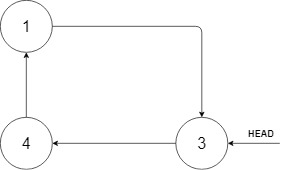
\includegraphics[width=150pt]{insert-into-a-cyclic-sorted-list-001.jpg}\\
\figcaption{before insert}\label{fig:insert-into-a-cyclic-sorted-list-001}
\end{center}

\begin{center}
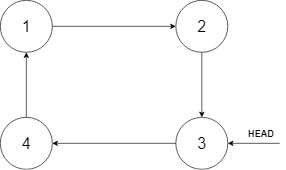
\includegraphics[width=150pt]{insert-into-a-cyclic-sorted-list-002.jpg}\\
\figcaption{before insert}\label{fig:insert-into-a-cyclic-sorted-list-002}
\end{center}

\subsubsection{分析}
Nil

\subsubsection{代碼}
\begin{Code}
// LeetCode
// 時間複雜度O(logn),空間複雜度O(n)
class Solution {
public:
    Node* insert(Node* head, int insertVal) {
        // edge case [1,1,1], target: 0
        // edge case [2,3,5,1], target: 0
        if (head == nullptr) {
            head = new Node(insertVal);
            head->next = head;
        }
        else {
            Node *cur = head->next;
            Node *prev = head;
            Node *pivot = nullptr;
            while (!(cur->val >= insertVal && prev->val < insertVal)) {
                if (prev->val > cur->val)
                    pivot = prev; // 找出邊界, case [2,3,5,1], target: 0

                prev = cur;
                cur = cur->next;

                if (cur == head->next) break; // 走了一個循環也沒有結果
            }
            if (cur == head->next && pivot)
                pivot->next = new Node(insertVal, pivot->next);
            else
                prev->next = new Node(insertVal, cur);
        }
        return head;
    }
};
\end{Code}


\subsubsection{相關題目}
\begindot
\item 無
\myenddot


\subsection{LRU Cache}
\label{sec:lru-cache}


\subsubsection{描述}
Design and implement a data structure for Least Recently Used (LRU) cache. It should support the following operations: get and set.

\fn{get(key)} - Get the value (will always be positive) of the key if the key exists in the cache, otherwise return -1.

\fn{set(key, value)} - Set or insert the value if the key is not already present. When the cache reached its capacity, it should invalidate the least recently used item before inserting a new item.


\subsubsection{分析}
為了使查找、插入和刪除都有較高的性能,我們使用一個雙向鏈表(\fn{std::list})和一個哈希表(\fn{std::unordered_map}),因為:
\begin{itemize}
\item{哈希表保存每個節點的地址,可以基本保證在$O(1)$時間內查找節點}
\item{雙向鏈表插入和刪除效率高,單向鏈表插入和刪除時,還要查找節點的前驅節點}
\end{itemize}

具體實現細節:
\begin{itemize}
\item{越靠近鏈表頭部,表示節點上次訪問距離現在時間最短,尾部的節點表示最近訪問最少}
\item{訪問節點時,如果節點存在,把該節點交換到鏈表頭部,同時更新hash表中該節點的地址}
\item{插入節點時,如果cache的size達到了上限capacity,則刪除尾部節點,同時要在hash表中刪除對應的項;新節點插入鏈表頭部}
\end{itemize}


\subsubsection{代碼}
\begin{Code}
// LeetCode, LRU Cache
// 時間複雜度O(logn),空間複雜度O(n)
class LRUCache{
private:
    struct CacheNode {
        int key;
        int value;
        CacheNode(int k, int v) :key(k), value(v){}
    };
public:
    LRUCache(int capacity) {
        this->capacity = capacity;
    }

    int get(int key) {
        if (cacheMap.find(key) == cacheMap.end()) return -1;

        // 把當前訪問的節點移到鏈表頭部,並且更新map中該節點的地址
        cacheList.splice(cacheList.begin(), cacheList, cacheMap[key]);
        cacheMap[key] = cacheList.begin();
        return cacheMap[key]->value;
    }

    void set(int key, int value) {
        if (this->capacity == 0) return;
        if (cacheMap.find(key) == cacheMap.end()) {
            if (cacheList.size() == capacity) { //刪除鏈表尾部節點(最少訪問的節點)
                cacheMap.erase(cacheList.back().key);
                cacheList.pop_back();
            }
            // 插入新節點到鏈表頭部, 並且在map中增加該節點
            cacheList.push_front(CacheNode(key, value));
            cacheMap[key] = cacheList.begin();
        } else {
            //更新節點的值,把當前訪問的節點移到鏈表頭部,並且更新map中該節點的地址
            cacheMap[key]->value = value;
            cacheList.splice(cacheList.begin(), cacheList, cacheMap[key]);
            cacheMap[key] = cacheList.begin();
        }
    }
private:
    list<CacheNode> cacheList;
    unordered_map<int, list<CacheNode>::iterator> cacheMap;
    int capacity;
};
\end{Code}


\subsubsection{相關題目}
\begindot
\item 無
\myenddot

\section{雙鏈表} %%%%%%%%%%%%%%%%%%%%%%%%%%%%%%

雙鏈表節點的定義如下:
\begin{Code}
// 雙鏈表節點
class Node {
public:
    int val;
    Node* prev;
    Node* next;
    Node* child;
};
\end{Code}

\subsection{Flatten a Multilevel Doubly Linked List}
\label{sec:flatten-a-multilevel-doubly-linked-list}


\subsubsection{描述}
You are given a doubly linked list which in addition to the next and previous pointers, it could have a child pointer, which may or may not point to a separate doubly linked list. These child lists may have one or more children of their own, and so on, to produce a multilevel data structure, as shown in the example below.

Flatten the list so that all the nodes appear in a single-level, doubly linked list. You are given the head of the first level of the list.

\begin{center}
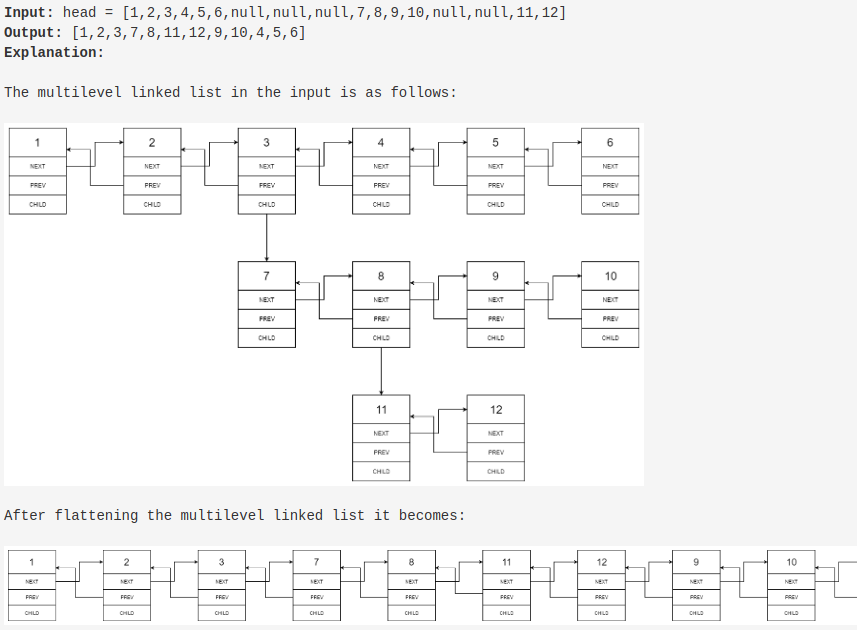
\includegraphics[width=300pt]{flatten-a-multilevel-doubly-list.png}\\
\figcaption{candy crush}\label{fig:flatten-a-multilevel-double-list}
\end{center}

\subsubsection{分析}
Nil

\subsubsection{遞歸版}
\begin{Code}
// LeetCode
// 時間複雜度O(n),空間複雜度O(1)
class Solution {
public:
    Node* flatten(Node* head) {
        for (Node *cur = head; cur; ) {
            if (cur->child == nullptr)
                cur = cur->next;
            else {
                cur->next = flatten_(cur->child, cur->next);
                cur->next->prev = cur;
                cur->child = nullptr;
            }
        }
        return head;
    }
private:
    Node *flatten_(Node* head, Node *tail) {
        Node *cur = head;
        while (cur->next) {
            if (cur->child == nullptr)
                cur = cur->next;
            else {
                Node *next = cur->next;
                cur->next = flatten_(cur->child, next);
                cur->next->prev = cur;
                cur->child = nullptr;
                cur = next;
            }
        }
        cur->next = tail;
        if (tail)
            tail->prev = cur;

        return head;
    }
};
\end{Code}

\subsubsection{Stack}
\begin{Code}
// LeetCode
// 時間複雜度O(n),空間複雜度O(1)
class Solution {
public:
    Node* flatten(Node* head) {
        if (head == nullptr) return head;

        stack<Node*> cache;

        Node *prev = nullptr;
        cache.push(head);
        while (!cache.empty()) {
            Node *cur = cache.top();
            cache.pop();

            if (prev)
                prev->next = cur;
            cur->prev = prev;

            if (cur->next) cache.push(cur->next);
            if (cur->child) cache.push(cur->child);
            cur->child = nullptr;

            prev = cur;
        }

        return head;
    }
};
\end{Code}

\subsubsection{相關題目}

\begindot
\item Nil
\myenddot
